\subsection{Ambiente de Software}
Para realizar o laboratório foi utilizado de algumas tecnologias e ferramentas são elas: 
\begin{itemize}
	\item \textit{Scikit}: é uma ferramenta de código aberto, simples e eficaz na análise de dados, acessivel e reutilizavel por vários contextos \cite{scikit-learn}. O projeto foi iniciado em 2007 com por intermédio de um projeto da Google Summer of Code, atualmente é mantido pela comunidade
	\item \textit{Python}: é uma linguagem de programação em script´s, interpretada, de código aberto e rápida, mantido pela comunidade e administrada pela Python Software Foundation. Diversas empresas já utilizam dela, como Google, YouTube e EVE Online.
\end{itemize}

\subsection{Base de dados}
Foi selecionada a base de imagens CKPLUS48. A qual pode ser encontrada em: https://www.kaggle.com/shawon10/ckplus. Contém 750 imagens de rostos em escalas de cinza com as expressões de raiva, nojo, desprezo, medo, felicidade, tristeza e surpresa. Para este laboratório foram selecionadas apenas as expressões raiva, medo, felicidade, tristeza e surpresa.

\subsection{Extração de características}

Para extração de características foi utilizado os descritores Local Binary Patterns (LBP) e o Gabor.

Sendo que o primeiro extrai 256 características de textura é não paramétrico, possui baixo custo de processamento \cite{rajan:19}. Seu funcionamento consiste em dividir a imagem em sub-blocos sendo que para cada sub-bloco é calculado o histograma, o vetor de características é formado com a concatenação desses histogramas \cite{rajan:19}.
Sendo que o segundo gera filtros com ondas senoidal, com os eixos desta onda busca encontrar a Gaussiana e assim manter uma proporção constante na imagem, para no final do processo gerar contornos e texturas para obter dados\cite{lima:2016}.Neste laboratório o Gabor extrai 60 características de textura como linhas e contornos nas imagens.
 
 Os arquivos finais podem ser encontrados em: \url{encurtador.com.br/gnDOZ}.

\subsection{Seleção dos classificadores e técnica de amostragem}
Os classificadores foram selecionados com base no trabalho de \cite{rajan:19}, o qual indica quais foram os mais utilizados em problemas de reconhecimento de expressões faciais (Facial Expression Recognition - FER), sendo eles:
\begin{itemize}
	\item \textit{Regressão Logística (Logistic Regression - LR)}: produz a partir de um conjunto de dados, modelos que permitem a predição por variaveis categóricas
	\item \textit{ K-Nearest Neighbors - (KNN)}: procura o vizinho K mais próximo de um dado ponto no espaço do conjunto de dados.
	\item \textit{Máquina de Vetores Suporte (Support Vectors Machine - SVM)}: é uma maquina de entrada e saida onde os dados que são enviados como entrada são mapeadas em um espaço multidimensional e encontra um hiperplano que separa os dados de entrada.
	\item \textit{Rede Perceptron Multicamadas (Multi-Layer Perceptron - MLP)}: é uma rede neural com camadas onde os números de neurônios são indeterminados, sendo assim não é possível prever a saída intermediaria entre as camadas.
	
\end{itemize}

 Para os experimentos executados nas seções seguintes o conjunto de dados foram divididos em 80\% para treino e 20\% para teste. A seleção desses subconjuntos foram feitos de modo aleatório com o número gerador  (\textit{seed}) 327 para possível reprodução dos experimentos.

\subsection{Seleção da técnica de normalização}

A partir dos arquivos gerados com os descritores foram alternadas as técnicas de normalização para verificar qual delas atinge melhor resultado para acurácia, métrica que calcula a razão entre quantidade de predições corretas e a quantidade de predições realizadas. 

As técnicas de normalização testadas foram:
\begin{itemize}
	\item \textit{Min-Max}: consiste em transformar cada característica com valor mínimo em 0 e os valores máximos em 1, sendo que o restante é transformado em um valor decimal entre 0 e 1.
	\item \textit{Standard}: são calculados a média e o desvio padrão da conjunto de amostras, em seguida é subtraída de cada amostra a média, o resultado então é divido pelo desvio padrão.
	\item \textit{Max Absolute}:é uma técnica parecida com o Min-Max porém, somente os valores absolutos e positivos são mapeados entre 0 e 1.
	\item \textit{Robust}: as estatísticas de mapeamento ocorrem pela escala de percentil, sendo assim aumenta a margem de onde estão os valores dos dados podendo ser até negativo, exemplo: -3 a 2.
\end{itemize}

\subsubsection{Descritor LBP}
A base CKPLUS com o descritor LBP apresentou pequena variação nos resultados como podem ser vistas na Figura~\ref{fig:bar_norm_all}.

\begin{figure}[!htbp]
	\centering
	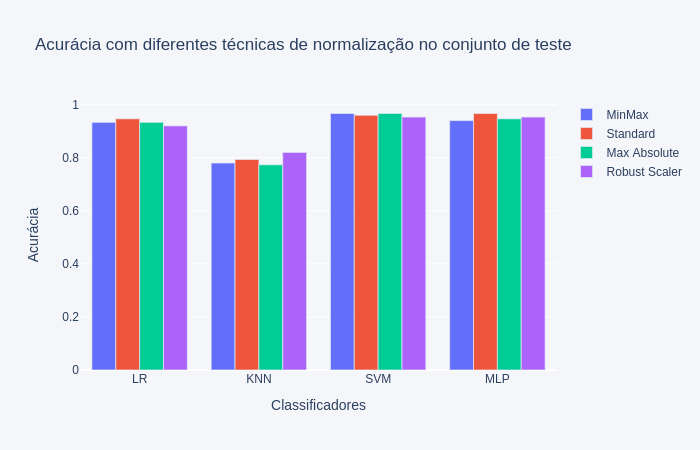
\includegraphics[width=1.0\linewidth,clip=true,trim=0cm 0cm 0cm 0cm, keepaspectratio=true]{bar_norm_all.png}
	\caption{Comparação de técnicas de normalização com descritor LBP.}
	\label{fig:bar_norm_all}
\end{figure}

Os classificadores MLP, SVM obtiveram os melhores resultados, 97\% de acurácia. Os piores resultados foram obtidos pelo classificador KNN, 77\%.

\subsubsection{Descritor Gabor}
Foram mantidos os classificadores e métrica utilizados no último experimento. Nenhum dos classificadores obtiveram 50\% de acurácia. Os resultados podem ser vistos na Figura~\ref{fig:bar_norm_all_gabor}.

\begin{figure}[!htbp]
	\centering
	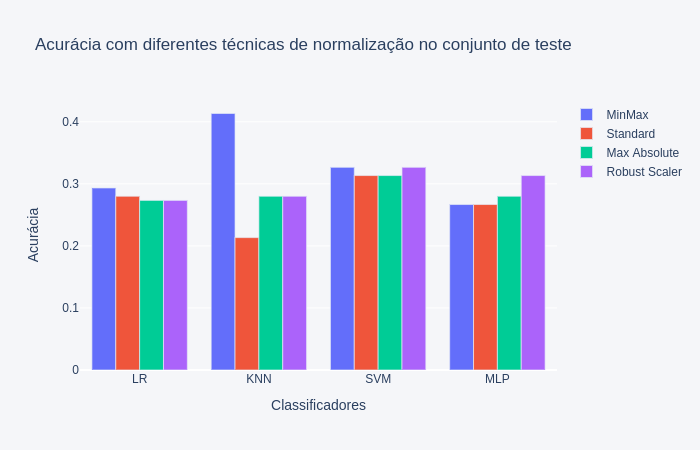
\includegraphics[width=1.0\linewidth,clip=true,trim=0cm 0cm 0cm 0cm, keepaspectratio=true]{bar_norm_all_gabor.png}
	\caption{Comparação de técnicas de normalização com descritor Gabor.}
	\label{fig:bar_norm_all_gabor}
\end{figure}

Pode-se observar que a técnica de normalização Min-Max, atrelado ao classificador KNN obteve o melhor resultado deste experimento, 41\%. Observa-se também que ocorre uma alta discrepância sobre os resultado obtidos entre os descritores LBP e Gabor.

\subsection{Redução de dimensionalidade}
\subsubsection{Descritor LBP}
Em seguida buscou-se reduzir a dimensão do conjunto de dados de modo a reter 90\% de variância. Primeiramente os dados foram normalizados utilizando a técnica \textit{Standard}, pois obteve resultado levemente superior no experimento anterior.

Com a técnica PCA para redução de dimensionalidade foi selecionado o menor número de componentes que retinha 90\% de variância. Foi possível reduzir de 256 para 133 característica. Ver Figura~\ref{fig:points_pca_lbp}. 

\begin{figure}[!htbp]
	\centering
	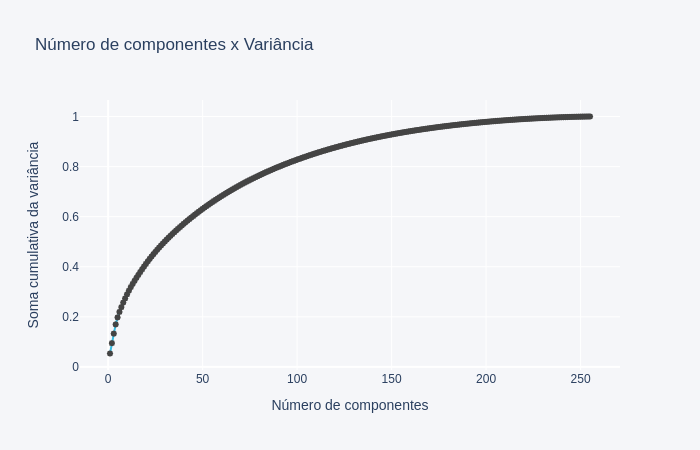
\includegraphics[width=1.0\linewidth,clip=true,trim=0cm 0cm 0cm 0cm, keepaspectratio=true]{points_pca_lbp.png}
	\caption{Selecionar o menor número de componentes retendo 90\% de variância.}
	\label{fig:points_pca_lbp}
\end{figure}

\subsubsection{Descritor Gabor}
Primeiramente foram normalizados os dados com a técnica \textit{MinMax} pois obteve o melhor resultado no experimento anterior. Ver Figura~\ref{fig:points_pca_gabor}.

\begin{figure}[!htbp]
	\centering
	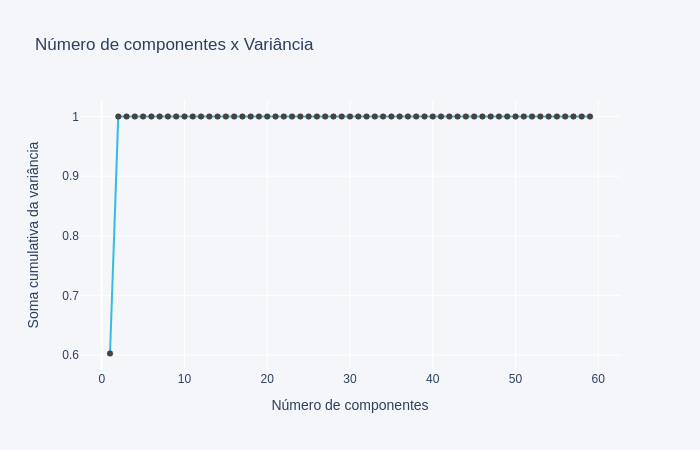
\includegraphics[width=1.0\linewidth,clip=true,trim=0cm 0cm 0cm 0cm, keepaspectratio=true]{points_pca_gabor.png}
	\caption{Selecionar o menor número de componentes retendo 100\% de variância.}
	\label{fig:points_pca_gabor}
\end{figure}

Observa-se melhores resultados comparado com o experimento anterior. Pois se fez possível reduzir as características de 60 para duas retendo 100\% de variância. Embora o desempenho dos classificadores atingirem no máximo 69.3\%, nota-se grande melhoria quando é reduzida a quantidade de características quando compara-se os resultados da Figura~\ref{fig:bar_norm_all_gabor} com a Figura~\ref{fig:bar_result_gabor}

\begin{figure}[!htbp]
	\centering
	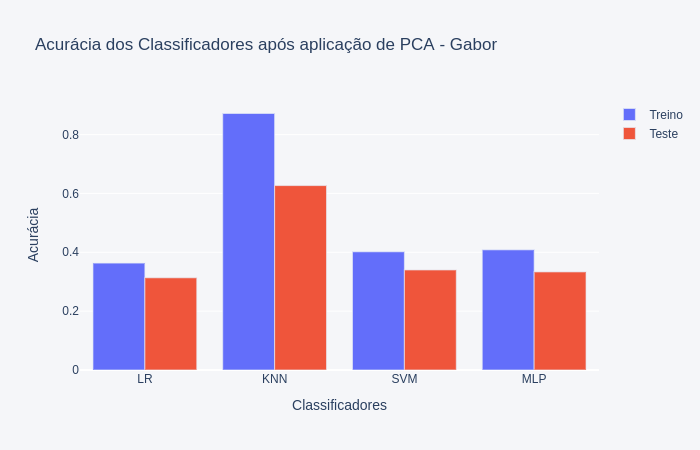
\includegraphics[width=1.0\linewidth,clip=true,trim=0cm 0cm 0cm 0cm, keepaspectratio=true]{bar_result_gabor.png}
	\caption{Acurácia com o descritor Gabor após redução de dimensionalidade}
	\label{fig:bar_result_gabor}
\end{figure}